% Created 2022-07-27 Wed 18:40
% Intended LaTeX compiler: pdflatex
\documentclass[11pt]{article}
\usepackage[utf8]{inputenc}
\usepackage[T1]{fontenc}
\usepackage{graphicx}
\usepackage{grffile}
\usepackage{longtable}
\usepackage{wrapfig}
\usepackage{rotating}
\usepackage[normalem]{ulem}
\usepackage{amsmath}
\usepackage{textcomp}
\usepackage{amssymb}
\usepackage{capt-of}
\usepackage{hyperref}
\author{Rushil Surti}
\date{\today}
\title{Notes: The Life of Pi}
\hypersetup{
 pdfauthor={Rushil Surti},
 pdftitle={Notes: The Life of Pi},
 pdfkeywords={},
 pdfsubject={},
 pdfcreator={Emacs 26.3 (Org mode 9.1.9)}, 
 pdflang={English}}
\begin{document}

\maketitle
\tableofcontents

\newpage

\section{Author's Note}
\label{sec:org800bf18}
The author of \emph{Life of Pi} is Yann Martel. In 1996, he released his second novel, and it was not received well, being quite unpopular. Martel then moved on to writing another novel in 1939, this time set in Portugal. As he did not have much money and was familiar with the region, Martel flew to live in Bombay, where he could live and settle down with less financial worry. Martel, dreaming a peaceful life of writing near a hill-side, began writing his third novel. In spite of the beauty of the characters, plot, and setting, Martel felt some emotional element was missing and was somewhat disheartened, and he ended up mailing away his notes to a fictional address. Martel, with even less money, decided to travel to South India. Martel then arrived at a town called Pondicherry, which was previously under rule by the French empire. At a place called the Indian Coffee House, Martel met a man, \uline{Francis Adirubasamy}, who was curious with his work and told him, "I have a story that will make you believe in God." At first, Martel did not believe him, but he relented and sat down to listen. The man mentioned the botanical garden's toy train tracks and how the train used to run twice an hour every day through the stations Roseville and Zootown. The man asked Martel to talk to the main character (of the book?) for his questions to be answered. When Martel went back to Toronto some time later, he called a certain Mr. Patel, the man Adirubasamy mentioned. The main character recalled his story and showed his diary and newspaper records to Martel. Martel then managed to get a tape from the Japanese Ministry of Transport. What Martel found did make him believe in God. This book, \emph{Life of Pi}, is the main character's story.
\section{Section 1: Toronto and Pondicherry}
\label{sec:org6bff5b4}
\subsection{Chapter 1}
\label{sec:org2861d00}
The main character attended the University of Toronto, majoring in both religious studies and zoology. For his zoology thesis, they chose to study the three-toed sloth.

One interesting point is that he said:
\begin{quote}
"I chose the sloth because its demeanour---calm, quiet, and introspective---did something to soothe my shattered self" (1.2).
\end{quote}
Coupled with the quote at the start of the chapter (seen below), it seems that the main character was unhappy with their life, only having religion and their interest in zoology.
\begin{quote}
"My suffering left me sad and gloomy" (1.1).
\end{quote}
The main character then goes on to explain certain findings of the three-toed sloth, being very truant and lazy, living in harmony with nature. The main character relates this to his belief of God.

Being a relatively good and prestigious student, the main character received awards and got along with his scientific peers, despite them being atheistic.
The main character comments little on his working life, only saying this:
\begin{quote}
"I have nothing to say of my working life, only that a tie is a noose, and inverted though it is, it wil hang a man nonetheless if he's not careful" (1.12).
\end{quote}
\textbf{Perhaps the main character has a somewhat unstable job or one that he has to carefully tread in?}

The speaker then laments a little, feeling homesick for his town in Pondicherry, India, but also reaffirms his love for Canada and how he would rather stay.

He then mentions that a certain man, \uline{Richard Parker}, stayed with him and that he misses him, seeing him in his dreams and nightmares. Richard Parker seems to have suddenly abandoned the speaker at some point in the past.

Abruptly, the setting seems to switch, with the speaker mentioning their time in a hospital in Mexico and the positive experience he had. The speaker was practically on the brink of death, barely able to walk with nausea and dizziness.

\textbf{What caused the main character to end up in the state? The events of the story? Why the sudden time leap?}

Next, the setting equally abruptly warps back to Canada, where the speaker laments how he was criticized for eating using his hands in an Indian restaurant.
\subsection{Chapter 2}
\label{sec:orgc81ea96}
This chapter solely describes a man living in Scarborough. The man is described as old, small, and thin, with dark hair and eyes. The man is also described to be expressive and straightforward in his speech.
\subsection{Chapter 3}
\label{sec:orgf984795}
One of the main character's father's business acquaintances by the name of Francis Adirubasamy, nicknamed Mamaji, was a friend of the family. This is the same man introduced in the author's note. The main character's brother, Ravi, used to joke about Adirubasamy's physical appearance, relating it to his love of swimming. Adirubasamy tried to teach swimming to the main character's family, but no one, besides the main character, was willing to learn. Eventually the main character went to the pool to practice and developed a love for swimming.

The main character then mentions Adirubasamy's ventures to Paris for studying. He then mentions the many pools that Adirubasamy visited during his time there, such as the Piscine Deligny, Piscine Château-Landon, Pisicine Rouvet, and others. Adirubasamy's favorite, however, was Piscine Molitor.

Because of Adirubasamy's love for it, the main character's name is \uline{Piscine Molitor Patel}.
\subsection{Chapter 4}
\label{sec:orgafae2b7}
The main character describes the formation of Zootown (also a name mentioned earlier in the Author's Note) due to Pondicherry entering the Union of India on November 1, 1954. The zoo was expansive and had a variety of wildlife.

Piscine mentions that, before the family moved to Pondicherry, his father used to work as a hotel owner in Madras. It is also revealed that the name of Piscine's father is Santosh Patel.

Piscine had fond memories of playing around in the zoo, seeing an exotic array of animals.

\textbf{Perhaps Piscine's love of animals contributed to his eventual pursuing of zoology from Chapter 1?}

Then, Piscine laments about the uneducated criticism zoos receive for "taking away the freedom" of the animals, which would supposedly be better off in the wild. He goes on to explain how this is not the case and living in the wild brings about constant pressure for survival. Animals are quite conservative and bothered by the smallest changes in their environment. Pisicne briefly relates this misunderstanding to religion and God.

The chapter ends with an explanation that the Pondicherry Zoo was filled in and discontinued.
\subsection{Chapter 5}
\label{sec:org739247f}
Due to the pronunciation of his name, Piscine met much teasing and bullying beacuse of its similarity to the word "pissing." Kids and teachers alike would mispronounce his name, by accident or by purpose.

When Piscine arrived at a new school called Petit Séminaire, an English-medium secondary school in which Ravi was already popular, he had a plan. When teachers called on him, Piscine went to the chalkboard and wrote:
\begin{quote}
My name is

Piscine Molitor Patel,

known to all as

Pi Patel
\end{quote}
He then wrote the constant \(\pi = 3.14\) and drew a circle with its diameter line. Doing this for every class with different teachers, he managed to avoid any teasing and made the trend catch on. Other students used greek letters such as \(\omega\), \(\upsilon\), \(\gamma\), \(\lambda\), and \(\delta\). The teasing stopped, and, as he referred to it, Pi found refuge.
\subsection{Chapter 6}
\label{sec:orgdca6864}
This is another odd chapter as it, like Chapter 2, very particularly details an unknown man. Perhaps as we continue reading, we will find out more information about this person to ascertain who he is.

The man is described as being a great cook, excelling at cuisine from any country. The man has a massive store of food.
\subsection{Chapter 7}
\label{sec:org3a55c20}
Pi has met a few people in his life that have changed his way of thinking. One of these people was his biology teacher, Satish Kumar. Mr. Kumar, a Communist of odd appearance, was a outward athiest, believing in science and reasoning over anything else. He would frequently come to the zoo to look at the animals.

One time, he saw Pi and call him over to talk. In a conversation between the two, Pi mentioned religion, and Mr. Kumar responded with "Religion? I don't believe in religion. Religion is darkness" (7.10). When Mr. Kumar was young, he was bedridden with polio. He prayed to God for help, yet no help came. Instead, medicine saved him.

As time went on, Mr. Kumar became one of Pi's favorite teachers. This caused Pi to realize that athiests are actually "brothers and sisters of a different faith" (7.20). Instead, Pi disliked agnostic people more for their indecisiveness and doubt at the center of their life.
\subsection{Chapter 8}
\label{sec:org1dc1cd5}
The chapter starts by stating that the most dangerous animals in a zoo are humans. Pi details this by recounting the many idiotic acts that people have done in zoos all around the world, such as feeding animals foreign objects like bottles, poisoning them, and fighting or harming them.

Pi's father, however, also believed there to be another, far more dangerous behavior: anthropomorphizing animals or treating them like they could be friends. To teach this lesson to Pi and Ravi, their father showed a hungry tiger viciously tearing into a goat in front of their eyes. The father then went on to explain that other animals, such as hippos, hyenas, ostriches, deer, camels, birds, and elephants are equally dangerous and should be treated with care.

The main idea to take away from the father's lesson is that \textbf{"[l]ife will defend itself no matter how small it is"} (8.85).
\subsection{Chapter 9}
\label{sec:org4c14d90}
One important part of taking care of animals is knowing something called their "flight distance," or the distance at which humans can approach animals with them still being comfortable. Some animals do not let you approach them, while others allow up to a certain distance.

Pi took pride in his father's natural gift of being able to judge the thought process and instincts of animals, allowing for him to judge their flight distance.
\subsection{Chapter 10}
\label{sec:org936ebc1}
Some zoo animals try to escape, not \emph{to somewhere}, but rather \emph{from something}. As earlier mentioned, animals are very susceptible to change, and the slightest inconvenience may cause them to try and leave. Even animals natively born in the zoo have some innate instinct to try to escape if their conditions are not met.

Regardless, many animals do not escape because, once again, they hate change, and the conditions out in the wild are unknown.
\subsection{Chapter 11}
\label{sec:org6f41b4b}
Pi explains, through the case of the escaped female black leopard of the Zurich Zoo, that many escaped, "dangerous" animals are in fact not harmful to society but simply creatures trying to survive. He also laughs at how many wild, exotic animals are potentially in big cities as opposed to what the populous might assume.
\subsection{Chapter 12}
\label{sec:orge7b649f}
Here, the story again (see Chapters 2, 6) vaguely mentions this character, thin, small chef character, but goes on to name him. The person that the chapter is referring to is Richard Parker, whom the reader was introduced to in Chapter 1, with Pi saying that Parker abandoned him.

\textbf{Who really is this man? What is his significance to the plot? Why did he and Pi split ways?}
\subsection{Chapter 13}
\label{sec:org1650b41}
The main character once again reiterates that, if someone were to fall into, for example, a lion pit, the lion would eat the person, not out of hunger or bloodthirst, but instead out of anxiety and protection of their territory.

Pi then goes onto show with the example of a circus trainer that animals, such as lions, follow a social hierarchy. Their place in the hierarchy determines their behavior and whether they feel inferior or superior to certain creatures. One way to appear higher in this hierarchy is to intimidate the animal and show that they do not own the territory by being there first. Coupled with loud sounds and such as a whip or a whistle, a lion or any other dangerous animal will likely stay away out of fear and uncertainty. If the lion is not sufficiently intimidated or does not know its place in the hierarchy, it remains alert and dangerous.
\subsection{Chapter 14}
\label{sec:org483700e}
Pi explains that the animal with the otherwise lowest ability or standing in a pack will make the most effort to build a close relationship with the keeper or the person with the highest standing. Animals do this in order to gain protection from stronger adversaries in the pack.
\subsection{Chapter 15}
\label{sec:org0b16682}
This chapter uses the same italic text and vague mention of "he," who we can assume to be the previously mentioned Richard Parker.

This chapter describes the house of Richard Parker, which is described as a temple. Throughout the house, there are remnants and objects from three different religions: Hinduism, Catholicism, and Islam. Instances of Hinduism can be found with statues and shrines of various gods such as Ganesha, Shiva, and Krishna. Catholicism is represented through a cross, a Bible, and depictions of Christ and the Virgin Mary. Islam is represented through the Arabic writing and a photo of Kaaba.

\textbf{Why does this Richard Parker character have these objects? Was he, like Pi, a religious researcher?}
\subsection{Chapter 16}
\label{sec:orgbf56ee9}
The start of the chapter opens with Pi explaining how he was taken to a Hindu temple at a very young age and how he was interested in Hinduism and religion ever since that time. Pi felt a strong tie to Hinduism, feeling a "presence" and a connection to it.

Pi then explains the Hindu persepective of the world, with the concepts of Brahman, reincarnation, karma, and liberation. At the end of it, Pi interestingly says that, despite how much devotion one has, they must not be too attached to God.

The chapter ends with Pi recalling an anecdote of someone mishearing "Hare Krishnas" as "Hairless Christians." Pi mentions this to reflect that it is not even wrong, and that many people, such as Muslims, Christians, and Hindus, all have something in common.
\subsection{Chapter 17}
\label{sec:org1819287}
In this chapter, Pi recounts his first interaction with Christianity in his trip to the hill station Munnar.

When Pi visited Munnar, he noticed three hills, each with their own building. The hill on the right had a Hindu temple. The one in the middle had a mosque, and the one furthest left held a Christian church. Curious about it, Pi went to the left hill to visit the church, arriving at the rectory. There, Pi saw how the doors to the priest and assistant's room were open and remarked at the comforting and welcoming environment. This deepened his interest in the church, causing him to go inside and question what he saw.

Later, Pi actually went in a talked to Father Martin, who told Pi the story of Christianity. First hearing it, Pi was quite confused about how God's Son paid the price for the sins of humanity. Pi was confused how God could die and why he would lower himself to the human level. It perplexed him more that God would not leave a descendant. When he questioned Father Martin about it, he replied that it was out of love.

All of these questions made Pi interested in the religion, and God would not leave his mind.

On the last day of Pi's stay in Munnar, he went to the church and asked Father Martin if he could be a Christian, to which he responded that Pi already was a Christian in his heart. Pi was delighted and made his way to the Hindu church to thank Krishna for introducing Jesus to him.
\subsection{Chapter 18}
\label{sec:org301fc95}
Pi encountered his third religion, Islam, at the age of fifteen. Pi was exploring the Muslim area of his hometown and passed by a mosque. Not daring to enter, Pi instead went past it and went into a poorer district, finding a shop. There, Pi saw some sort of bread or dough and went to inspect it. The owner of the shop then appeared and asked Pi if he would want one. Pi, startled threw the piece of food on the ground. Despite this, the owner asked if he would like another one, to which Pi obliged, and they ate together.

After they finished, the owner started to explain how the bread was made but was interupted by the muezzin, a person who calls upon Muslims to pray. The owner fetched a carpet and began the ceremony right in front of Pi, doing, what seemed to Pi, interesting stretches and exercises.

This left an impact on Pi, who was left, just like with Christianity, curious.
\subsection{Chapter 19}
\label{sec:orgbeada4e}
Pi went back to the bread shop owner and inquired about his religion. When asked what it was about, the owner responded that "'It is about the Beloved,' [\ldots{}]" (19.3). Pi realized that Islam was about brotherhood and devotion.

Pi then recounted his positive experience of praying with the rest of the worshippers.
\subsection{Chapter 20}
\label{sec:org73c86d0}
Pi described the owner's relationship and devotion to God as personal and loving. Pi remarked this as a bit interesting because the owner's name, Satish Kumar, was the same name of his Communist, athiest biology teacher. Pi accredited his love of zoology and his love of religion to the two Satish Kumars.

Pi felt the presence of and a deep connection to God while praying at the owner's shop. Pi had this same feeling later in Canada. After snow had fallen during the night, Pi had to trek his way up to a house during the day. As he ventured towards it, he saw movement and looked around. In front of his eyes, he envisioned the kind, loving Virgin Mary. Pi felt rewarded with the presence of God.
\subsection{Chapter 21}
\label{sec:orgf370b61}
This chapter is quite cryptic in its meaning. The style again reverts to the italic text, signifying that this involves Richard Parker somehow.

Pi, presumbably, after having met with Richard Parker, felt down about the contentment of his life, which Parker described with, "'dry, yeastless factuality', 'the better story'" (21.1). Pi then writes on paper an equally cryptic message.

\begin{quote}
"Words of divine consciousness: moral exaltion; lasting feelings of elevation, elation, joy; a quickening of the moral sense, which strikes one as more important than an intellectual understanding of things; an alignment of the universe along moral lines, not intellectual ones; a realization that the founding principle of existence is what we call love, which works itself out sometimes not clearly, not cleanly, not immediately, nonetheless ineluctably. [\ldots{}] An intellect confounded yet a trusting sense of presence and of ultimate purpose" (21.2,4).
\end{quote}

The paragraph seems to describe religion and a more moral, emotional view as opposed to a scientific or intellectual view. I am not fully sure what these words mean or how they relate to the story.
\subsection{Chapter 22}
\label{sec:org962ceb6}
Pi believes that, in their last moments, an athiest will see a blinding light and relent in belief to God; whereas, an agnostic, which Pi describes with the words, "dry, yeastless factuality" (22.1), the same words from the previous chapter, would try to explain this warm light with science or reasoning and miss out on something.
\subsection{Chapter 23}
\label{sec:orgd628211}
On one day, three people of high status from the Christian, Hindu, and Islam communities went to see Pi and his family. Pi, not having told his family or others that he was practicing three religions, was worried. Pi's father was not religious at all, and his mother was likely neutral. As the three men approached Pi and realized the others, they were confused and somewhat angry. While the parents were also surprised, they did not seem to be angry. The three began to argue over their religions. As Pi's father tried to calm them down, Pi was forced to speak up. Pi quoted Gandhi in saying that "all religions are true" and that he wanted to love God. Not being able to argue with a well-meaning child, the three men backed off.
\subsection{Chapter 24}
\label{sec:org439e3e1}
Ravi makes fun of Pi for his interest and following of multiple religions.
\subsection{Chapter 25}
\label{sec:org19d7b2c}
Pi laments the state of those that rush to defend God against any sort of disrespectful language. Pi does not believe that God is so fragile to need the outward, public defense of humans. Instead, Pi believes that God needs to be defended on the inside, in people's hearts.

Pi states that he was chased away from a mosque, glared at by a priest, and shooed away from darshan. After the public finds out that Pi follows three religions, they believe that Pi is betraying them. Pi, on the other hand, does not understand this behavior because chasing him away from religious practices does not do God any good.

Despite the opposition Pi faces, he still continues to practice all three religions.
\subsection{Chatper 26}
\label{sec:org5a4989b}
One day, Pi works up the courage to confront his family about the situation.

Pi asks his father for a baptizing and a prayer rug, wishing to practice Hinduism, Christianity, and Islam at the same time. When asked why he wants to pray, Pi responds that he loves God. His father still does not relent and explains that he does not have to practice three religions, but Pi says that he wants to. When Pi's father says that he cannot follow all three religions at once, Pi disagrees. In a classic father move, Pi's father tells Pi to talk to his mother about it.

Pi confronts his mother with the same request. Pi's mother says to talk to his father about it, but Pi informs her that he already did. Pi's mother then tries to distract Pi with a book to read, but Pi sees through her. Pi's mother explains that they do not understand Pi's enthusiasm for religion and that she does not believe that Pi can follow three religions at once. Pi relates religions to nations and manages to somewhat win the argument with his mother, who relents.
\subsection{Chapter 27}
\label{sec:org288dd0d}
This chapter details a conversation between Pi's father and mother following the events of Chapter 26.

The two parents once again reiterate that they do not understand Pi's obsession with religion as they are both very modern. The two then go on to talk about their displeasure with Mrs. Gandhi, who they describe as foolish and something that will pass.

\textbf{Note: Here, the parents use a very interesting piece of figurative language, describing India and Pi, in his own way, as "marching to the drumbeat of progress."}

The conversation moves on to the parents criticizing Pi's addressing of Gandhi as "Bapu," which is quite affectionate, as well as his following of Islam. While his father finds Hinduism fine and Christianity tolerable, he does not quite accept Pi becoming a Muslim due to how different they are. In the end, though, the parents give up and label it as hopefully just being a phase.
\subsection{Chapter 28}
\label{sec:orga01981e}
Pi talks about his love of his prayer rug and his peaceful experience praying outside in the yard. Pi would pray in the direction of Mecca with his face to the floor. Sometimes, a member of the family would look at him as they were getting used to the sight.

Pi also recounts his baptism, which his mother and father attended.
\subsection{Chapter 29}
\label{sec:org97f0f07}
Pi outlines the chapter by stating at the beginning that people move out of hope for better conditions.

Pi, who did not care much for current events at the time, explains the political struggles of the time period that caused his father and mother a great deal of worry. The Tamil Nadu government, a major critic of Mrs. Gandhi, had been taken down, marking the ever approaching dictorial takeover.

Pi explains that "bad politics is bad for business" (29.7). The zoo was not making much money as is, so the changing of rights and removal of democracy only served to worsen the situation.

Pi then reiterates on the first paragraph by explaining that people move out of anxiety.

Soon, Pi's parents told Ravi and him that they would be moving to Canada, a country almost on the other side of the world.
\subsection{Chapter 30}
\label{sec:org3878144}
Here, we see the italic text appear, indicating a time shift.

The chapter opens with Pi introducing his wife, Meena, to the mystery narrator. The narrator then describes the condition of their home and Pi's characteristic shyness.

\textbf{Question: Originally, I thought the vague narrator here to be Richard Parker, this mysterious person who we were not given much information about, but could the narrator here be the author instead?}
\subsection{Chapter 31}
\label{sec:orgf013729}
Pi invited Mr. Kumar, the baker, to the zoo. Worried that he would miss Mr. Kumar for how plain of a person he was, Pi kept on close watch outside the main gate and ignored friends coming his way.

Once they met, Pi waived any payments for him and invited him in. Mr. Kumar was quite fascinated by the animals, liking the zebra in particular. Along the way, they met the other Mr. Kumar, the teacher.
\subsection{Chapter 32}
\label{sec:orga8adf03}
In this chapter, Pi explains the phenomenon of zoomorphism, where animals treat humans or animals of different kinds as their own kin. Pi gives a few examples, such as a rat and vipers coexisting in the zoo until an unaware young cobra bit it as well as the lion cub with a dog mother.

Pi explains that the reason for zoomorphism is not well known, but he believes that: "the answer lies in something I mentioned earlier, that measure of madness that moves life in strange but saving ways" (32.9).
\subsection{Chapter 33}
\label{sec:orgbdc75a3}
This chapter once again features the italic text.

Perhaps continuing from the last "time skip" chapter, the narrator is shown photos of Pi's life. There are pictures from the wedding, honeymoon, his university, and graduation. Interestingly, the narrator remarks, "A smile every time, but his eyes tell another story" (33.1).

There are also photos from Brazil and places over the Pacific, but those pictures were lost. Another picture depicts a major political figure visiting the zoo.

Another picture shows schoolchildren, with Pi pointing one of them out to be Richard Parker.

\textbf{Note: Originally, I thought the mysterious narrator was Richard Parker, but this solidifies the fact that it is most likely the author, Yann Martel.}

At the end of the chapter, Pi laments that he cannot remember his mother clearly.
\subsection{Chapter 34}
\label{sec:org5add0b8}
This chapter details the selling of the zoo, the main preparation for the family's trip to Canada.

The animals were mostly sold to other zoos all across the United States, but a select few ended up in Canada. Pi details that moving the animals and trading them involved extensive paperwork and caused quite a bit of stress for his father.

Along the way, Pi and Ravi felt that they did not want to move to Canada.

Pi was first introduced to Americans when they came to inspect the condition of the animals.
\subsection{Chapter 35}
\label{sec:orga2b8294}
\begin{center}
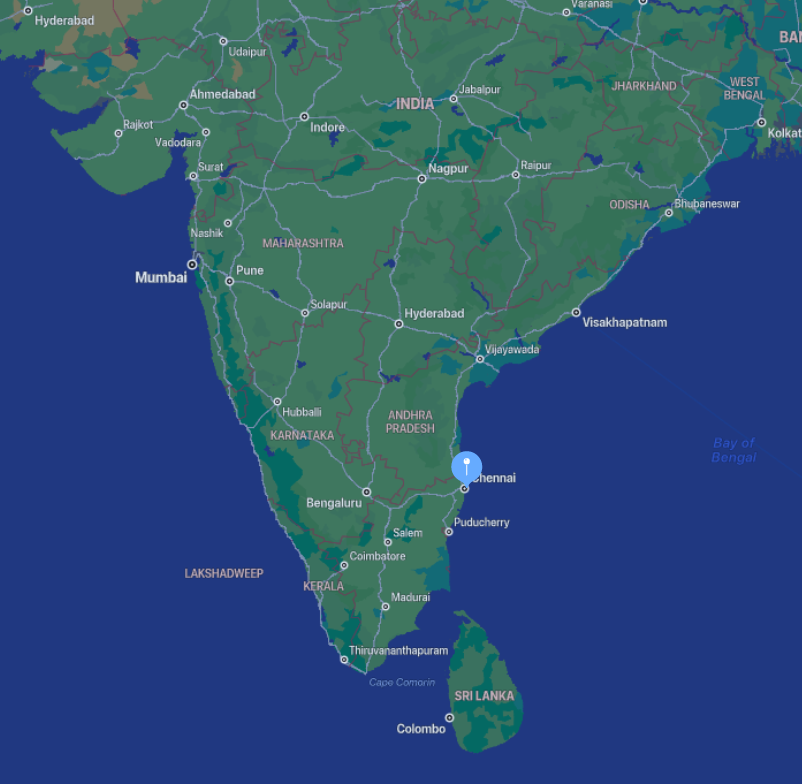
\includegraphics[width=.9\linewidth]{./img/madras.png}
\end{center}
Pi's family prepared to leave from Madras on June 21st, 1977 on the large cargo ship \emph{Tsimtsum}. As the animals were sedated and loaded on to the ship, the family said their goodbyes to everyone, and the ship started moving. Despite Pi's original hesitancy towards moving, he noted that he was quite excited.

At the end of the chapter, Pi states that "[t]hings didn't turn out the way they were supposed to\ldots{}" (35.6).

\textbf{Note: This may foreshadow future conflict.}
\subsection{Chapter 36}
\label{sec:org402acff}
This chapter is again in the "time leap" style.

This time, the narrator goes into Pi's house, meeting his son, Nikhil, his daughter, Usha, his dog, Tata, and his cat, Moccasin. This chapter almost confirms that the narrator is the author when Nikhil says, "'Dad! The writer's here'" (36.3).

The narrator tries talking to Usha, who is shy and hides behind Pi's leg. Pi explains that Usha is four years old. Pi plays with her, causing her to laugh, ending the chapter happily.
\section{Section 2}
\label{sec:orgf0cbc13}
\subsection{Chapter 37}
\label{sec:org0db48b6}
The ship sunk, and Pi was separated from his family. From the lifeboat, Pi saw Richard Parker in the water, on the verge of drowning.

\textbf{Note: Although Richard Parker has been directly referenced a few times throughout the story, it seems that we still do not know much about him. What is his relationship to Pi? When Pi is yelling at him, he says that Parker is a strong swimmer. Perhaps Parker is a friend of Adirubasamy?}

While refusing to accept the current situation, Pi urges Parker to swim to the boat. After a while of trying, Pi's personality suddenly switches and he tries in vain to force Parker away. Despite this, Parker still makes it onto the boat. Here, we learn that Parker is not a human but rather a three year old adult tiger.

Pi falls overboard in shock as to what he has just done.
\subsection{Chapter 38}
\label{sec:org48b1437}
\begin{center}
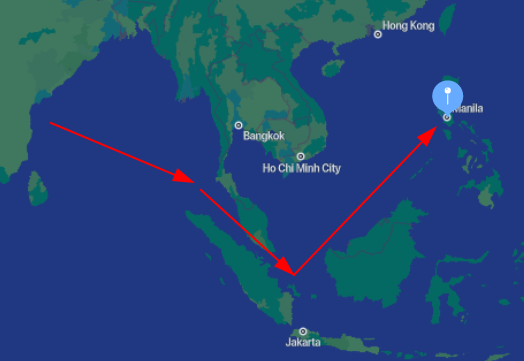
\includegraphics[width=.9\linewidth]{./img/route_to_manila.png}
\end{center}
At first, the journey of the ship was fine. The ship made its way safely to Manila, where it stopped for animal feed, cargo, and ship maintenance. Pi watched the animals, but Ravi watched the men working on the ship. Ravi told Pi that there was something wrong with the engine.

A little while after they set sail again, Pi heard an explosion in the early morning. Pi tried to wake up Ravi to no avail and thought better than to wake up his parents, so he went to explore alone.

Pi made his way upstairs to the main deck and found that there was some light rain. As Pi looked around, he did not see anything out of the ordinary except for the lifeboat being out of place. The ship was tilting. Pi felt the need to go back.

After going down one level, he saw that it was full of water. Despite his family being below, he rushed upstairs to safety. Pi realized the ship was sinking and began looking for other people, while running into animals.

Pi ran to where the officers would be, but did not find anyone. There were, however, three crew members. As Pi tried to talk to them, he was handed a life jacket and tossed overboard.
\subsection{Chapter 39}
\label{sec:org0bbab65}
When Pi was thrown overboard, he landed on the lifeboat, losing his life jacket. Instead of the crew jumping in after him, a zebra jumped out, hit the bench of the lifeboat, and sent it falling into the ocean.
\subsection{Chapter 40}
\label{sec:org26dab1f}
This chapter continues the events of Chapter 37.

Pi falls into the water overboard after saving Richard Parker, the tiger. Using the oar and lifebuoy as floating devices, Pi manages to float a few feet into the air, out of the reach of the sharks in the water.
\subsection{Chapter 41}
\label{sec:orge7e80a5}
In order to get a better vantage point, Pi cautiously pulls himself up onto the boat. Although he does not see any other lifeboats or survivors, he does survey the situation of the boat. 

The zebra is lying on the floor with a broken leg, but still living, to the surprise of Pi who thought it would have been eaten by the tiger. Pi then looks past the zebra and sees a hyena. Pi surmises that the hyena was always there, the tiger must have fallen off, and that the crew who threw him overboard earlier were not doing so to save him but instead to use him as bait.

The weather then clears as the day begins.
\subsection{Chapter 42}
\label{sec:orgc355f9f}
"Orange Juice," the orangutan, floats in the direction of the boat, standing on a net covered with spiders and bananas. As the orangutan makes its way onto the boat, the net begins to sink. Pi picks up the net, which is hinted to be useful later on in the future, but does not manage to pick up the bananas, which he regrets later on.

Still being quite confused with the situation, the orangutan lays on the tarpaulin of the boat for a minutes before falling onto the body of the lifeboat. This beckons a scream from the hyena.
\subsection{Chapter 43}
\label{sec:org3812c5c}
Pi holds out hope that rescue ships or other vessels will soon come to rescue his family and him. Pi then explains the situation on the boat.

The zebra generally lies still throughout the duration of the chapter. The hyena, however, does anything but. It runs in circles around the boat, resting only at a few periodic intervals. Although the hyena comes close, it does not interact with Pi, who is on edge, both figuratively and literally.

Pi explains the true nature of a hyena. Although they look cowardly and air-headed during the day, they become true hunters at night, ganging up on any prey they can find. Pi also explains that hyenas have little to no morals, eating or doing anything that they please, limited only by their jaw strength.

At the end of the chapter, the hyena stops and lays down near the zebra.
\subsection{Chapter 44}
\label{sec:org6a8c082}
As the sun sets and night falls, Pi loses vision of what is going on. Fearing that the hyena will go after him, Pi tries to stay on the very edge of the boat. Although the animals make sounds, the boat does not move, and Pi is not harmed.

Eventually the night passes.

\textbf{Question: How long will Pi be able to hold on to the oar? How will he go about acquiring food and clean water?}
\subsection{Chapter 45}
\label{sec:orge8cea30}
As day breaks out again, Pi finds hope in and believes that, this day, he will be rescued. Peering into the boat, Pi sees that the hyena attacked the zebra at some point, biting off its broken leg.

Pi shifts his position on the oar, moving closer to the hyena, and is able to see the orangutan. Pi notes its human-like seasickness and lack of injury.

A sea turtle then appears, bumping into the boat. Pi says that he would befriend this species later on. After a few minutes, the turtle leaves.
\subsection{Chapter 46}
\label{sec:orgf67303d}
Pi begins to lose hope of rescue, telling the reader that this night was one of his worst nights ever. On the boat, Pi notices that the orangutan, Orange Juice, has an expression that shows it has committed to death.

After the hyena wakes up and moves, it eats the zebra, ripping off its skin and eating its insides. The orangutan, startled, gets up and begins to roar. The hyena roars in response. The zebra's blood also attracted sharks, who hit the boat. Despite this situation, nothing happens.

After the sun sets, Pi finally accepts that help is not coming and that his family is dead.
\subsection{Chapter 47}
\label{sec:org22cb054}
Despite its injuries, the zebra is still alive but barely able to move. The other two animals are both on edge.

The zebra dies a few hours later in the afternoon. The hyena charges the orangutan, but the orangutan hits it on the head. Pi feels instilled with hope, but he knows that the orangutan cannot win against the hyena. The hyena beheads the orangutan and faces Pi. Before thowing himself on the hyena, Pi looks down, sees Richard Parker, and collapses.
\subsection{Chapter 48}
\label{sec:orgdfacc65}
Pi explains the story of how Richard Parker got its name from a shipping mixup between a professional hunter, Richard Parker, and a tiger cub he caught, who was suppsed to be called Thirsty. Instead, the papers the zoo received had the hunter as "Thirsty" and the cub as "Richard Parker."
\subsection{Chapter 49}
\label{sec:orgbe9ff72}
Pi has not had food or water for the past three days. Pi's thinking begins to slow, and he has trouble moving. Because of this, Pi, having nothing to lose, crawls inward on the boat, searching for water.

Pi also reflects on the past behaviors of the animals, now making much more sense due to the presence of Richard Parker.
\subsection{Chapter 50}
\label{sec:orge315f54}
Pi scans the area of the boat, noting the measurements of various items, and finds items such as life jackets, buoys, and oars.
\subsection{Chapter 51}
\label{sec:orgd4b70ac}
In search of water and food, Pi moves inward towards the boat, concocting a plan to get under the tarpaulin without Richard Parker noticing. Eventually, Pi finds a locker containing canned water and packages of food.

Using the hooks of the tarpaulin to open the can, Pi drinks four containers of water and feels invigorated. Pi then begins to feel hungry. He opens a package of biscuits, which are made out of wheat, animal fat, and sugar.

Pi takes record of the contents of the locker. There are thirty-one containers of food left, each meant to last three days. This equates to 93 days worth of food. Pi also has enough water to last at least 124 days.
\subsection{Chapter 52}
\label{sec:orgd5d6303}
Pi lists out all of the supplies found in the locker.

\begin{itemize}
\item 192 tablets of seasickness medicine
\item 124 cans of water
\item 32 plastic vomit bags
\item 31 cartons of food rations
\item 16 wool blankets
\item 12 solar stills (used for making fresh water out of salt water via evaporation)
\item 10 life jackets
\item 6 morphine syringes (pain-killers?)
\item 6 hand flares
\item 5 oars
\item 4 parachute flares
\item 3 large plastic bags
\item 3 can openers
\item 3 glass beakers
\item 2 boxes of matches
\item 2 smoke signals
\item 2 plastic buckets
\item 2 plastic bailing cups (used for removing water from a boat?)
\item 2 airtight plastic containers
\item 2 sponges
\item 2 long, buoyant ropes
\item 2 short, non-buoyant ropes
\item 2 fishing kits
\item 2 gaffs (iron hooks for fishing)
\item 2 anchors
\item 2 hatchets
\item 2 rain catchers
\item 2 pens
\item 1 cargo net
\item 1 lifebuoy
\item 1 hunting knife
\item 1 sewing kit
\item 1 first-aid kit
\item 1 signalling mirror
\item 1 pack of cigarettes
\item 1 bar of chocolate
\item 1 survival manual
\item 1 compass
\item 1 notebook
\end{itemize}

Pi eats a quarter of the chocolate bar, examines the rain catchers, and goes to sleep.
\subsection{Chapter 53}
\label{sec:org96bb08c}
Pi realizes that his life is in danger with Richard Parker aboard the boat. Discovering that he has a strong will to live, he thinks of ways to avoid Richard Parker and survive. Quickly, Pi begins crafting a raft out of oars, buoyant rope, and the lifebuoy.

As Pi is crafting the raft, Richard Parker, just a few feet away from Pi, finally kills the hyena. Richard Parker turns his gaze towards Pi.

Suddenly, a rat appears and attaches itself onto Pi's head, further drawing Richard Parker's attention. As Richard Parker slowly encroaches closer on Pi, Pi throws the rat into his mouth as an offering, which satisified the tiger.

As Richard Parker goes back to eat the hyena again, Pi quickly finishes the raft, noting Richard Parker's seasickness. The raft, although small, floats perfectly, but Pi is wary of sharks or waves potentially stranding him.

The day quickly starts to end, and rain begins falling. Pi pulls himself up onto the boat to fetch a rain catcher, a bag, and a blanket. In the process of doing so, he slams the locker, annoying Richard Parker. Pi falls back to the raft.
\subsection{Chapter 54}
\label{sec:org8f2a219}
Pi roughs out the rainy, windy night.

During the night, he goes over plans in his head to get rid of Richard Parker. After pondering and eliminating unreasonable plans, Pi decides to wait out the life of Richard Parker, who does not have a steady supply of food and, more importantly, water.
\subsection{Chapter 55}
\label{sec:org6a5dc94}
Pi wakes up as the rain stops and realizes the vastness of the ocean.

Pi also goes over his plan to wait out Richard Parker's life, but he realizes that tigers can drink saline water from the ocean, and, as Richard Parker gets more hungry, he will lash out at Pi and eat him out of desperation.
\subsection{Chapter 56}
\label{sec:orgb293d27}
Pi spends this chapter talking about the effect of fear on the body, how it leads to doubt and lack of trust, and how you must fight it. Pi regards fear as life's true opponent.
\subsection{Chapter 57}
\label{sec:org6608705}
As Pi is on the raft, Richard Parker lets out a sound called prusten, which "expresses friendliness and harmless intentions" (57.5). Pi is surprised and realizes that he can assert dominance over Richard Parker and tame him like a circus trainer would.

Pi acts out and yells lines like a circus trainer while blowing a whistle. This irritates Richard Parker and succeeds in pushing him back.

Instead of waiting out the tiger's health, Pi decides that he will change the plan and keep Richard Parker alive. Pi says that he actually does not want Richard Parker to die because he would then be left alone to face despair.
\subsection{Chapter 58}
\label{sec:org398c5ff}
Pi reads the survival manual, which contains some basic tips for surviving after a shipwreck.

Afterwards, Pi sets out a few tasks to complete for himself:

\begin{itemize}
\item Train Richard Parker.
\item Start fishing food for Richard Parker.
\item Create a canopy for the raft.
\item Tie a second rope from the lifeboat to the raft.
\item Improve the raft.
\item Stop blindly hoping and be more active.
\end{itemize}

At the end of the chapter, Pi cries, thinking that his situation is quite grim.
\subsection{Chapter 59}
\label{sec:orgabf9112}
Pi notices that, with the raft acting as an anchor, the lifeboat has switched directions. This works out for Pi because it intensifies Richard Parker's seasickness.

As Pi returns to the lifeboat for supplies, he observes a party of cockroaches jumping off the lifeboat to their death, leaving only Pi and Richard Parker to be left on the boat.

Pi enters the tarpaulin and, upon seeing a pool of rainwater, drinks it to preserve what he has left. 

Pi then begins work on the raft, adding a second rope, creating a mast and canopy, and installing solar stills.

While the sun sets, Pi observes the wide variety and density of life in the ocean.
\subsection{Chapter 60}
\label{sec:orga22e97b}
While observing the scene around him at night, Pi contemplates his suffering and relates it to a Hindu story he has once heard.
\subsection{Chapter 61}
\label{sec:org7faf47d}
This chapter, Pi attempts fishing for food for Richard Parker.

At first, Pi tries using his last leather shoe as bait, but he ends up expending it without catching anything.

After having a minor internal crisis about his plan to keep Richard Parker alive, Pi looks inside the locker for something to use as bait when he is suddenly hit by a flying fish. Pi tries feeding it to Richard Parker, but the fish flies away. Afterwards, however, a school of flying fish and dorado appears near the boat, some flying over, some landing on the boat itself.

Both Richard Parker and Pi caught a few flying fish.

Pi rushes back to the raft to prepare the fish but cannot bring himself to kill them with the hatchet. Instead, Pi breaks their necks. Pi is distraught with what he has brought himself to do.

Using the fish's head as bait, Pi manages to catch a dorado, which is much larger. This time, Pi happily hacks away at it with his hatchet, somewhat realizing that he is used to killing now.

The chapter ends with Pi feeding the dorado to Richard Parker and going to sleep, planning to fish more.
\subsection{Chapter 62}
\label{sec:org71a9a1b}
In this chapter, Pi tackles the problem of Richard Parker's, as well as his own, thirst.

After pondering for a bit, Pi turns towards the solar stills with doubt. To his surprise, all of them were full of fresh water, totaling around eight liters.

Pi drinks one container's worth and gives the rest, with some salt water added, to Richard Parker. During this, Pi realizes that the lifeboat has turned into a miniature zoo.

Pi tries his luck at catching more fish but does not succeed.

At the end of the chapter, Pi states that the next morning will mark exactly one week after his ship, the \emph{Tsimtsum}, sunk.
\subsection{Chapter 63}
\label{sec:org39ad3e8}
Pi states that he lasted 227 days stranded at sea, from July 2nd, 1977 to February 14th, 1978.

Pi then goes over his daily routine. Any small changes could greatly affect the routine. In addition, Pi did not keep track of the time passing. As such, he did not remember everything in order.

\subsubsection{Sunrise to Mid-Morning}
\label{sec:orge4c245e}
Pi wakes up, prays, makes breakfast for Richard Parker, inspects the vessels, cares for the solar stills, eats breakfast, and fishes.

\subsubsection{Mid-Morning to Late Afternoon}
\label{sec:org5e66ccd}
Pi prays, eats lunch, and participates in recreational activities.

\subsubsection{Late Afternoon to Early Evening}
\label{sec:org8428c18}
Pi prays, fishes, examines curing flesh, and prepares and eats dinner.

\subsubsection{Sunset}
\label{sec:org5382a65}
Pi inspects the vessels once again, collects any water from the solar stills, stores food and equipment, makes arrangements for sleeping, and finally prays.
\subsection{Chapter 64}
\label{sec:org1392592}
Pi recalls his clothes slowly disintegrating into nothing, leaving him to deal with salt-water boils.
\subsection{Chapter 65}
\label{sec:org61924d6}
\begin{center}
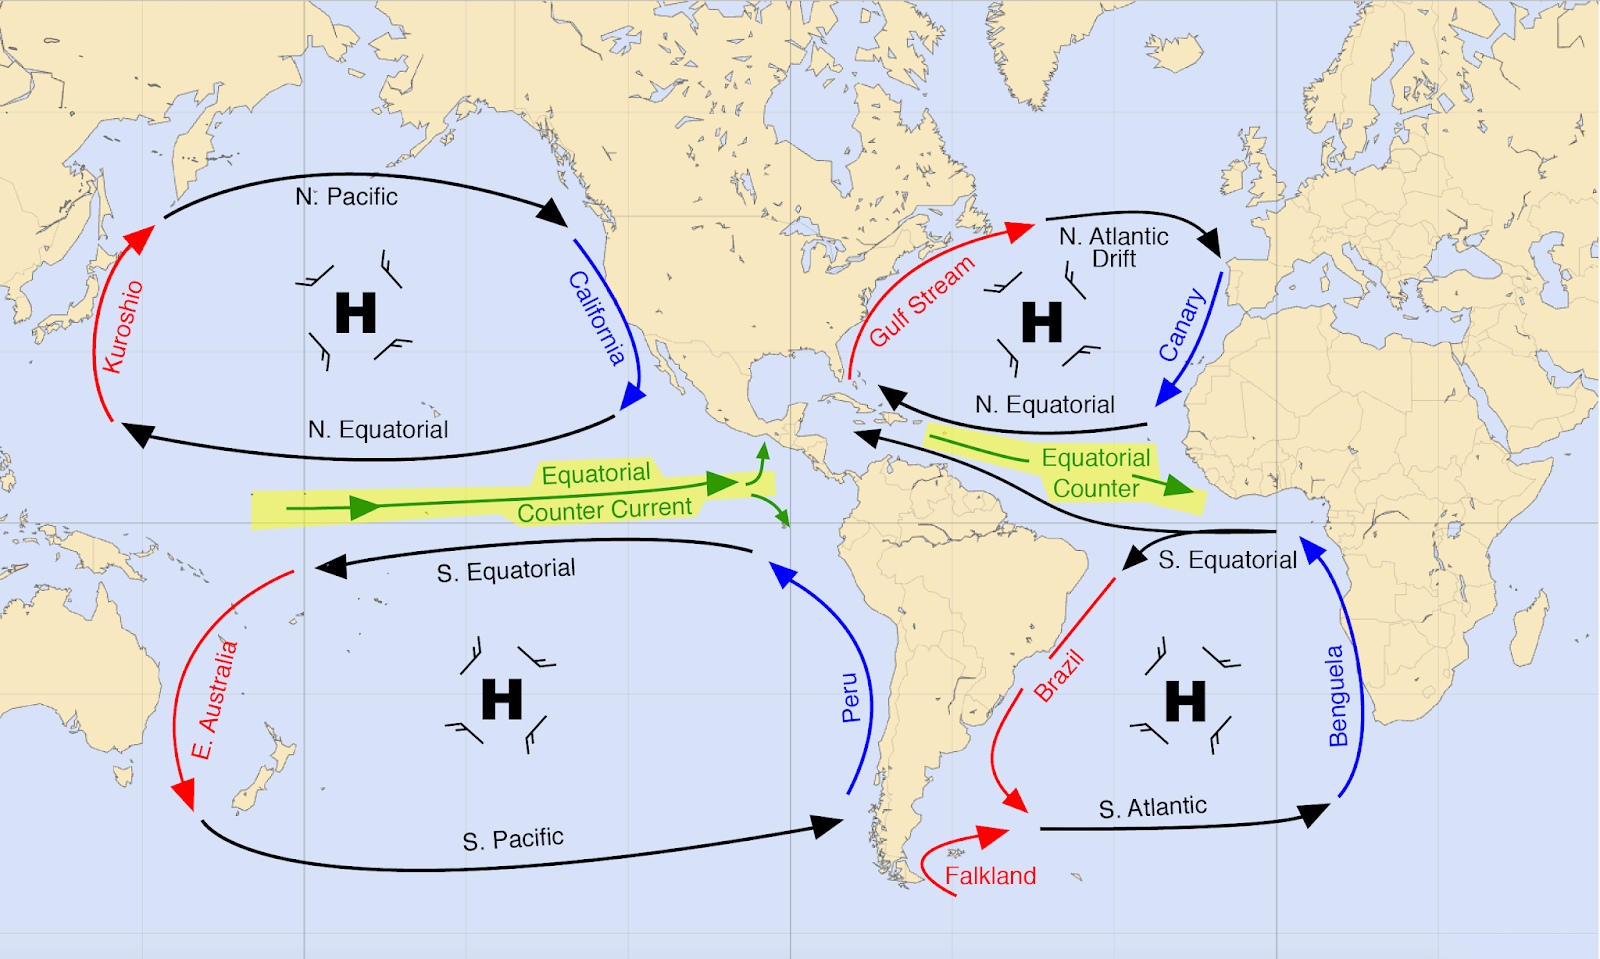
\includegraphics[width=.9\linewidth]{./img/equatorial_countercurrent.png}
\end{center}

Pi laments his lack of knowledge of navigation, wind currents, and marining in general. He does not know where or how to guide the boat, so he drifts, going along with the winds.

At the end of the chapter, future Pi mentions that he was travelling along the Pacific equatorial counter-current, highlighted in the picture.

\textbf{Question: Going based off of the map, will Pi end up somewhere in Central America?}
\subsection{Chapter 66}
\label{sec:org7e58d35}
In this chapter, Pi details more of his fishing accolades.

Pi quickly becomes more accustomed to hunting fish, using strategies such as wounding their gills so that they swim up and disguising the fishing hook with a net covered with seaweed.

Pi also details his struggle in catching turtles. Although they are slow and easy to stop, Pi found difficulty in hauling them onto the ship due to their near insurmountable weight.

Pi once again reflects on his actions, labelling himself as a savage.
\subsection{Chapter 67}
\label{sec:org25cc6da}
Pi talks about the marine life building up on the raft and lifeboat, consisting of algae, small shrimp, translucent fish, worms, slugs, barnacles, and crabs.

Pi eats everything but the worms and remarks that only the crabs tasted good.

Pi also watches the marine life as a way to pass time.
\subsection{Chapter 68}
\label{sec:orgd0bc555}
Pi details how his sleep schedule changed. Due to anxiety, Pi only ever slept for around an hour at a time continuously.

Richard Parker, on the otherhand, was able to sleep quite soundly in various different positions.
\subsection{Chapter 69}
\label{sec:org547a8b8}
Pi recalls his attempts to use flares to signal for help. In the end, none of them prove successful, to the point where Pi gives up on being saved.

Pi realizes he needs to find land.
\subsection{Chapter 70}
\label{sec:orge05bca9}
Pi manages to bring the turtle onto the lifeboat without bothering Richard Parker. As the survival manual suggests, Pi cuts its neck artery and collects the blood that comes out of it, only amounting to a can's worth.

In order to stop it from moving, Pi tries to cut off the head of the turtle, which does not work. Pi then decides to give the remaining body of the turtle to Richard Parker as food.

Pi, disappointed with the amount of work that he has to do in order to get such a measly amount of blood, thinks about how to best handle Richard Parker from now on.

Pi ends the chapter by saying, "It was time to impose myself and carve out my territory" (70.7).

\textbf{Inference: From this quote, we can most likely tell that Pi will try to further tame Richard Parker and establish his own territory in an effort to make Richard Parker respect him.} 
\subsection{Chapter 71}
\label{sec:orgcc00c81}
Pi outlines his plan that he uses to tame Richard Parker.

Pi blows his whistle to stir up Richard Parker and bait him into entering his "territory." After Richard Parker sets foot into this space, Pi increases his volume in order to show Richard Parker that he is very territorial.

Pi then controls the lifeboat to increase the waves and thus the seasickness of Richard Parker. By doing this and repeating the steps, Richard Parker gradually associates the whistle with severe nausea and seasickness. Pi then makes sure that Richard Parker does not sustain harm from the seasickness.

In this way, Pi can control the behavior of Richard Parker.
\subsection{Chapter 72}
\label{sec:org30060d5}
This chapter details Pi's initial struggle in taming Richard Parker.

Pi confronts Richard Parker with a heavy turtle shell as a shield. As he begins to make noise, Richard Parker swipes his paw at Pi, knocking him off of the lifeboat and into the water. This happens four times in total before Richard Parker succumbs to the whistle.

Pi explains that he is not harmed because, like most predators, Richard Parker does not actually want to engage in fights that could be deadly.
\subsection{Chapter 73}
\label{sec:org527a314}
In this chapter, Pi describes his longing for a book or religious scriptures.

Pi also states that he started writing a diary around a week after the \emph{Tsimtsum} sank. The entries are not labelled with dates.
\subsection{Chapter 74}
\label{sec:orgcf00722}
Despite the circumstances, Pi tries his best to continue his prayers and devotion to religion.

Although at times Pi feels grim, he tries to cheer himself up and continue loving God.
\subsection{Chapter 75}
\label{sec:org0846827}
Pi celebrates what he estimates to be his mother's birthday.
\subsection{Chapter 76}
\label{sec:orge03ee88}
Pi describes his routine of cleaning up after Richard Parker's excrement. Pi explains that this was done to prevent infection as well as assert dominance over Richard Parker. Because Richard Parker hides it from Pi, Pi can sense that the tiger is intimidated by him.

Pi laments that, due to low water and high protein intake, both Richard Parker and him are constipated.
\subsection{Chapter 77}
\label{sec:orgd6db06d}
As Pi's original rations begin to run out, he resorts to eating less, but this only increases his hunger. Pi relishes the sea life that he catches and begins to eat them more desperately. During this time, Pi develops a strong dislike towards salt.

Pi is gradually driven to a point of almost madness where he tries to eat the feces of Richard Parker. It holds no nutritional value, and Pi spits it out.

Eventually, parts of Pi's body, especially his legs, begin to decay.
\subsection{Chapter 78}
\label{sec:orgedcc0b8}
Pi describes the plentiful different sceneries present in the sky and sea.

Pi also makes a few connections to his life as a castaway.

Pi believes that "[t]o be a castaway is to be a point perpetually at the centre of a circle" (78.5). Pi says that, although the colors and the brightness changes, the shape stays the same. He is also constantly between the sun and the moon, both circles.

Pi also believes that being a castaway entails experiencing many extreme opposites: the bright, scalding, dryness of the day and the dark, shivering, dampness of the night. Pi also describes the opposites of boredom and terror, which play with the mind.

Pi relates his situation to an endgame in chess. The pieces are simple and few, but there is much risk.
\subsection{Chapter 79}
\label{sec:orgff5d67f}
Pi retells his experience with sharks on the lifeboat.

The sharks, mostly consisting of makos, blue sharks, and oceanic whitetips, do not bother Pi or the lifeboat for the most part.

Pi begins to catch some sharks for food. The first shark he catches is a mako. Pi flings it onto the lifeboat and into Richard Parker's territory. There, Richard Parker claws at it, and the shark bites into his paw. The two creatures fight, and while Richard Parker is victorious, he does sustain some temporary damage.

After that experience, Pi starts catching smaller sharks.
\subsection{Chapter 80}
\label{sec:orgb9ba21f}
One day, during a storm of flying fish, Pi catches a dorado on the lifeboat with a gaff. Pi, delighted, finds himself approached by Richard Parker, who also seems to want the dorado.

Pi and Richard Parker stare each other down, and, to Pi's surprise, Richard Parker relents. With this, Pi feels that he has tamed Richard Parker.

With this knowledge, Pi gradually stays on the lifeboat for longer and becomes used to being around the tiger.
\subsection{Chapter 81}
\label{sec:org15c3cc5}
Pi also explains that Richard Parker does not attack him because he provides the security of food and water. Richard Parker does not have many other reliable ways of acquiring resources, so to kill Pi would be to kill Richard Parker.
\subsection{Chapter 82}
\label{sec:orgcfc36c6}
As Pi safeguards the solar stills in the locker, Richard Parker's and Pi's supply of food and water steadily begins to deplete.

Pi tries to scavenge for all the water he can get, and he quickly catches food and prepares it to give to Richard Parker.
\subsection{Chapter 83}
\label{sec:org6bc8502}
Pi encounters a harsh storm with heavy waves.

While riding out the storm, the lifeboat as well as Pi and Richard Parker sustain damages. The raft is reduced to only a few floating oars, and the tarpaulin is torn apart.
\subsection{Chapter 84}
\label{sec:org7752b12}
After the storm, Pi encounters new wildlife in the form of whales, dolphins, and various types of birds.

Unfortunately, the birds are migratory birds, and they do not hint at the lifeboat approaching land.
\subsection{Chapter 85}
\label{sec:orga75281e}
Pi sees lightning hit water close to the lifeboat and is struck with wonder.
\subsection{Chapter 86}
\label{sec:orged022e0}
The lifeboat passes right by an oil tanker. Pi tries to fire a flare but aims it poorly and misses. Pi attempts other ways of grabbing the vessel's attention, but they all fail.
\subsection{Chapter 87}
\label{sec:orgdac5f37}
Pi puts a cloth over his face while sleeping, causing him to experience abnormal dreams due to asphyxiation. Pi does this to pass time.

\textbf{Note: Do not try this at home.}
\subsection{Chapter 88}
\label{sec:orge5b4365}
Pi encounters man-made debris and trash in the ocean. Pi takes an empty bottle, but otherwise, nothing of use is found.

Pi puts in an emergency message in the empty bottle and throws it into the ocean.
\subsection{Chapter 89}
\label{sec:orgfde5b73}
Pi describes the salt and sun induced decaying of everything: the lifeboat, clothes and blankets, Richard Parker, and Pi.

Pi and Richard Parker lose large amounts of weight and mostly pass the days by resting for long periods. Pi writes his last diary entry due to running out of pens.
\subsection{Chapter 90}
\label{sec:org32b2f7e}
Both Richard Parker and, eventually, Pi lose their vision.

As Pi resigns himself to death and lies down, he hears what he believes to be Richard Parker talking to him. Shortly after, Pi realizes that the voice is coming from another stranded person on another lifeboat. They discuss about food and other matters for a while with Pi referring to the person as "Brother."

After talking, the two try to find each other in their mutual blindness and converse a bit more, telling stories and dreaming of food. Eventually, they tether the boats together.

As the two meet and embrace, the man puts his hands on Pi's throat, planning on killing Pi for food. Before Pi can warn him, however, Richard Parker claws the man, killing him.
\subsection{Chapter 91}
\label{sec:org57d24ed}
Pi scavenges in the person's ship, finding the food and water. In addition, because of his tears, Pi's vision gradually returns.

Pi is forced to use some of the human flesh for fishing and food.
\subsection{Chapter 92}
\label{sec:orgf8c12f2}
Pi, still starving and thirsty, discovers a several square-mile island made fully out of algae, housing trees. Pi is able to eat the sugary algae and the fresh water it produces, giving him the energy to recover.

Richard Parker, too, ventures onto the island and quickly gets used to it, though he remains somewhat anxious. Richard Parker recovers, to the worry of Pi, who believes that the tiger may grow more confident and less respectful of Pi. Richard Parker returns to the lifeboat each night after Pi.

After Pi grows healthy enough to walk and explore farther, he comes across plains home to thousands of meerkats. The meerkats are friendly, and the plains also feature ponds of freshwater.

Interestingly, the meerkats swim into the freshwater ponds and return with large fish. Pi surmises that this is due to the saltwater ocean fish dying due to freshwater. Pi also sees Richard Parker in the distance killing an abundance of meerkats. The meerkats are not scared.

Pi cleans the lifeboat and tries to explore the entire island to no avail. Pi, however, does note the change of the algae due to the temperature of the day. In addition, Pi notices that the island holds up well against the elements. This makes him question the lack of other wildlife.

One day after Pi has a dangerous encounter with the reinvigorated Richard Parker, he decides to train Richard Parker again.

As Pi gets more used to the island, he decides to sleep on it, avoiding the lifeboat. Pi makes a makeshift hammock and sleeps in the trees. One day, however, Pi is woken up by the meerkats to see that a striking number of fish and even sharks are deposited in the ponds. After Pi goes back to sleep for a while longer and wakes up, he sees that the dead marine life is no longer there. Pi, not believing this to be the work of the meerkats nor Richard Parker, is puzzled.

Another day, Pi encounters a tree that seems to have a fruit. After climbing up the tree to acquire it, he realizes that the fruit is not a fruit but rather a ball of leaves. After unwrapping the leaves, he finds a human tooth. Pi finds more of these leaf fruits, each of them containing a tooth. In total, they complete a full set of 32 human teeth.

Pi has his doubts but tries one last experiment in order to confirm them. At night, Pi puts his foot onto the algae and sees that the algae is, in fact, acidic, and the island is, chillingly, carnivorous. This explains the death of the fish and sharks and Richard Parker's reason for returning to the lifeboat every night.

Pi decides that he and Richard Parker need to leave the island. After Richard Parker returns in the night, the anchor rope is dissolved, and the two leave the island.
\subsection{Chapter 93}
\label{sec:orgc788468}
Pi says that, "[t]he rest of this story is nothing but grief, ache and endurance" (93.1). Despite this though, Pi feels optimism and turns towards God.
\subsection{Chapter 94}
\label{sec:orgc3b15fe}
The lifeboat comes ashore in Mexico. Much to Pi's disappointment, Richard Parker leaps off the boat and heads to the jungle without much acknowledgment of Pi and without a formal goodbye.

After a few hours, people find Pi and take care of him, cleaning him, feeding him, giving him clothes, taking him to a hospital, and eventually getting him a foster parent, leading to his university life.

Pi expresses thanks to all of the people who made his life possible.
\section{Section 3}
\label{sec:org701d7bd}
\subsection{Chapter 95}
\label{sec:org0bd4c38}
The setting is stated to be Benito Juárez Infirmary, Tomatlán, Mexico.

Tomohiro Okamoto, a head in the Japanese Ministry of Transport, and his colleague, Atsuro Chiba, take a long journey down to Tomatlán, Mexico to speak with Pi, the sole survivor of the sunken ship, the \emph{Tsimtsum}.

The next chapter is a transcript of the conversation that they have.
\subsection{Chapter 96}
\label{sec:orgc83ecf4}
Okamoto and Chiba introduce themselves to Pi, set up a tape recorder, and ask Pi to recount the entire story. The date is Februrary 19th, 1978.
\subsection{Chapter 97}
\label{sec:orgbc188f3}
The story.
\subsection{Chapter 98}
\label{sec:orgda6267f}
After Pi recounts his story, the two men interviewing him are, somewhat understandably, doubtful of its legitimacy.
\subsection{Chapter 99}
\label{sec:org75b5a39}
Pi and the two interviewers debate on the validity of Pi's story regarding topics such as the floating bananas, algae island, tiger, meerkats. Pi ends up putting up quite the fight and strongly refutes their arguments, all the while gradually, and comedically, taking their lunch.

Eventually, the two ask Pi for a story without animals that does have any "invention." Pi somewhat maliciously complies, crafting a fake story of how four people, his mother, a cook, a sailor, and him, managed to get onto the lifeboat. Pi tells a story full of drama with an evil cook and much bloodshed. Interestingly, however, the people in the story seem to bear a resemblance to some of the animals in Pi's original story.

The two inquire more about the ship itself and what might have caused it to sink, but nothing is brought to light.

Pi asks the two which story was better, to which they reply stating that they like the one with the animals better.

Pi says that he will move on and go to Canada.
\subsection{Chapter 100}
\label{sec:org3e7d77a}
The last chapter contains the report published by Mr. Okamoto.

In the report, Okamoto details the information Pi gave him regarding the sinking of the ship.

At the end of the report, Okamoto writes about the strength and courage of Pi, including a reference, surprisingly, to Pi's original story through the mention of "an adult Bengal tiger" (100.5).

\section{Analysis}
\label{sec:org284ff75}
\subsection{Character Development}
\label{sec:org76f5669}

For the most part, we see Pi and Richard Parker as the only dynamic characters of the story. For the short while that Pi's family, relatives, friends, and acquaintances appear, we don't quite see a substantial amount of growth or learning compared to Pi. As Pi is an adolescent, this makes sense and might be the reason why this is a popular youth novel.

\subsubsection{Pi's Growth}
\label{sec:org956b47d}

Pi's growth starts even before the sinking of the \emph{Tsimtsum} and his ordeal on the lifeboat. In the first part of the story, we see a curious, impressionable, and young version of Pi. Because of these qualities, Pi picks up valuable knowledge from the people around him.

Pi learns a great deal from his interest in religion, with the teachers of each religion instilling life lessons, hope, and excitement.

At a young age, Pi picks up swimming from a man named Adirubasamy, a friend of his father. Pi gains a respect for the man and is infused with his passion of swimming and love of the ocean.

Because Pi's father is the owner of a zoo, Pi's acquires a love of nature and a deep insight into the thought process and behavior of animals.

It is clear that much of Pi's encounters in his early life were critical for his later survival on the lifeboat, the setting where much of Pi's growth and maturity comes from.

After the \emph{Tsimtsum} sinks, Pi is left stranded on a lifeboat with only a few other animals, one being a Bengal tiger. He loses his family in the process and finds that no help comes for in the following days.

In response to his endlessly grim circumstances, Pi still finds hope and does not resign himself to death. Over time and in spite of hardships, Pi builds mental strength and finds a strong will to live. This speaks highly to the fortitude and toughness of his character and hints at quite a deal of reflection.

One particular point in the story where this is apparent is when Pi makes the decision to leave the algae island. Despite the abundance of resources and prospects of survival, Pi pushes forward in search of land instead of living out his days stranded and alone like the person before him. Pi acknowledges that there will be struggle and grief, but he decides to leave anyways. In making such a decision, Pi exhibits an enduring conscience.

In addition to this mental fortitude that he builds, Pi learns essential survival skills in a trial-by-fire sense. Pi experiences what it is like to build shelter, acquire food and water, and fight for survival.

\subsubsection{Richard Parker's Growth}
\label{sec:orga183c00}

Richard Parker, another one of the main characters of the story, grows and develops alongside Pi, although less subtly.

As the story progresses, Richard Parker becomes more friendly with Pi and gains a respect for him as an "alpha animal." Like Pi, Richard Parker grows to accept the conditions around him and does not give up on living.

By the end of the story, Richard Parker runs into the jungle, never to be seen by Pi again, but he does not leave as the same tiger. Richard Parker leaves Pi having lost everything yet starting anew, stronger than ever.

\subsection{Conflict Development}
\label{sec:org03e9a92}

At the beginning of the story, Pi lives out his life rather peacefully.

The first minor conflict for him would be his unusual name, garnering him a somewhat unpleasant reputation at school. This type of conflict aligns with a more typical youth novel.

The second minor conflict Pi experiences is his parents' and others' aversion to Pi believing in three religions, Hinduism, Christianity, and Islam.

These two conflicts are "man versus society" type conflicts.

Finally, the last conflict that Pi faces in the early parts of the book is dealing with the thought of moving to Canada, a far away country. This conflict aligns more towards "man versus self" in dealing with emotions and "man versus man" in that his parents are the cause of the conflict.

The real main conflict starts, quite obviously, with the sinking of the \emph{Tsimtsum} and the Pi's harsh striving on the lifeboat. This entire quest is an example of "man versus nature" as Pi fights to survive Richard Parker, the climate, starvation, and dehydration.

\subsection{Symbolism}
\label{sec:orga21cbb4}

Despite supposedly being a real story, \emph{The Life of Pi} does contain some symbolism.

In fact, one outright example of symbolism is the made-up story that Pi tells the two interviewers at the end of the book. Pi projects the animals on the boat onto people in this false story. Pi symbolizes Richard Parker's mean, ferocious appearance as an evil, cannibalistic cook. The zebra with the broken leg represents the sailor, who also had a broken leg. The hyena who, for a time at least, coexisted with the tiger represents Pi's mother.

Another great example of symbolism appears with Pi's encounter of the algae island. In my opinion, the algae island represents something of a false paradise, akin to a mirage oasis in a desert, although slightly different. Pi is miraculously saved by the island, but he soon finds that not everything is as it seems.

Another good way to look at the algae island is to view it as a materialization of complacency. As Pi lives some days on the island, he is forced to confront the decision of whether or not he should leave. After seeing the remains of a dead human, however, Pi is reminded of the dangers of not moving on. Pi ponders what kind of life that person must have lived through, how lonely it must have been to waste away until their death.

Before it is destroyed, the raft symbolizes a safe haven or a home for Pi. Pi is separated from Richard Parker, has shelter, and is free to carry on whatever he wants to do without any obstruction. On the raft, he eats; on the raft, he sleeps.

\subsection{Critical Thinking}
\label{sec:org9e3eb05}

Some possible questions to have in mind.

\begin{itemize}
\item How does religion affect Pi's view of the world and help him on the lifeboat?
\item How does Pi grow as a character throughout the story?
\item Why do you believe Yann Martel, the author, included parts of Pi's early life before the sinking of the \emph{Tsimtsum}?
\item Why do you believe Yann Martel chose to intersperse parts of Pi's future as an adult as the story progressed?
\item What is the significance of the interview at the end of the story?
\item Why do you believe the author chose to write chapters of such varying length?
\end{itemize}

\subsection{Thoughts}
\label{sec:org1b39935}

Overall, I actually quite enjoyed the book, and I feel that this was a nice opportunity to finally read and analyze the classic story that I had only vaguely heard of. Although some parts, such as the introduction, did drag on, I found that the short chapters helped to keep my attention and interest me.

In my opinion, a lot of this book seems to feel like a "love letter to God." Although not stated outright, the story seems to flow in a beautiful way that really focuses on Pi's love for religion and how it impacted his life.

The book is very philosophical and psychological at times, understandably so, due to just how emotionally moving and changing Pi's situation is. It is clear that Pi spent a lot of his time thinking and reflecting on the state he is in.

\emph{Do I think that the story really is real?} To be honest, it is really hard for me to say. I know quite little about the behavior of animals and the legitimacy of a carnivorous, so I cannot comment on that part. However, even though the purely logical side of me is saying that a tale so coincidental and miraculous is statistically very unlikely, another part of me cannot shake the feeling that it would not necessarily be impossible. Whatever the case, the lesson that the book carries is powerful and is, for me, the most important takeaway from this book.

Do not lose hope.
\end{document}
